\chapter{Chapter ~\ref{ch:modeling-evaluation} Aditional Plots}
\label{ap:aditional-plots}


In this appendix, we include some plots generated by the study presented in Chapter~\ref{ch:modeling-evaluation}, which have been cut off and not included in the final text version. They are:

\begin{itemize}
	
	\item CDF's distributions;
	
	\item QQPlots;
	
	\item Cost history ($J_\nabla$) and data linearization from linear regression;
	
	\item Other plots for $AIC$, $BIC$ and $J_M$.
	
\end{itemize}

\clearpage

\begin{figure}[ht!]
	\centering
	\label{fig:aproximation-original-cdf-bigFlows}
	\subfloat[Cauchy]{
		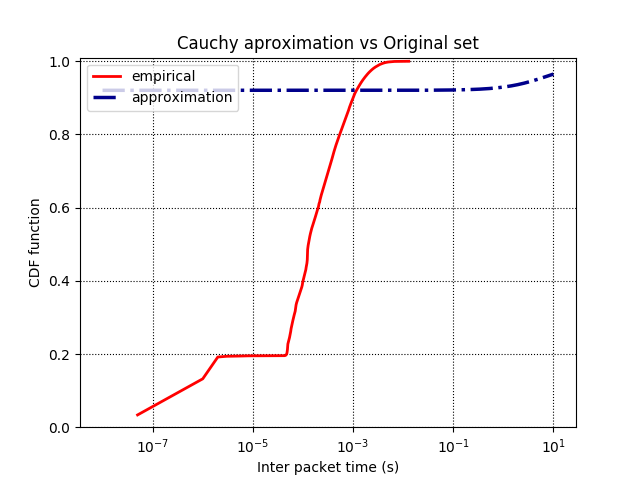
\includegraphics[width=62mm]{figures/apC/cdf/bigFlows_Log_-_Cauchy_aproximation_vs_Original_set}
	}
	\subfloat[Exponential(LR)]{
		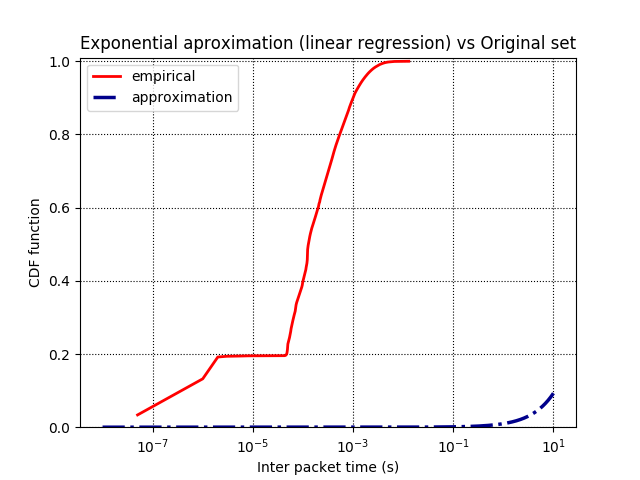
\includegraphics[width=62mm]{figures/apC/cdf/bigFlows_Log_-_Exponential_aproximation_(linear_regression)_vs_Original_set}
	}
	\hspace{0mm}
	\subfloat[Exponential(Me)]{
		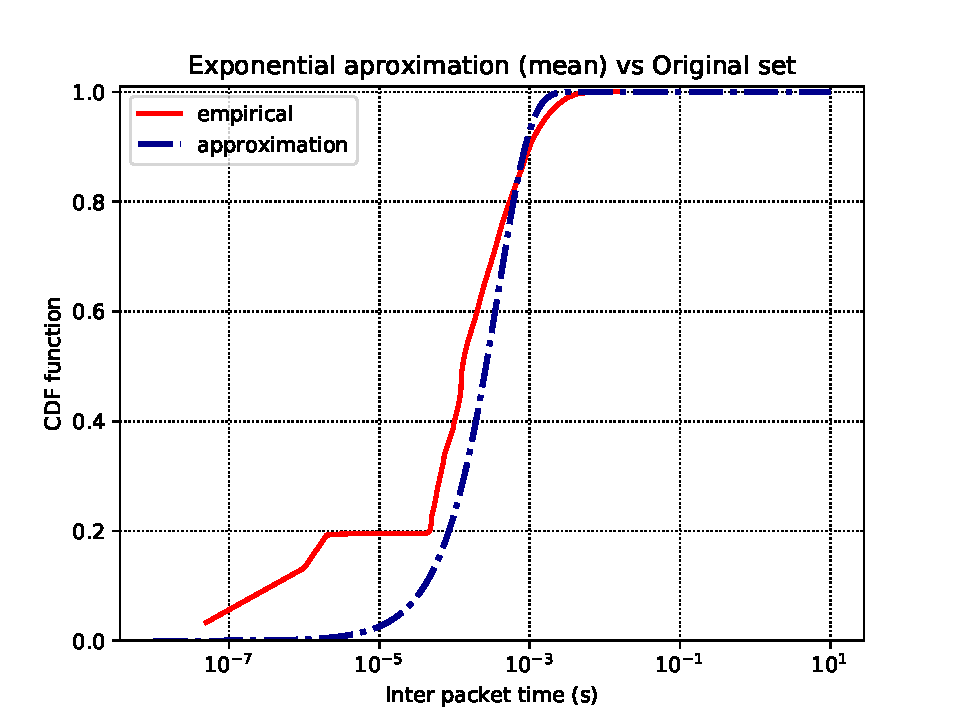
\includegraphics[width=62mm]{figures/apC/cdf/bigFlows_Log_-_Exponential_aproximation_(mean)_vs_Original_set}
	}
	\subfloat[Normal]{
		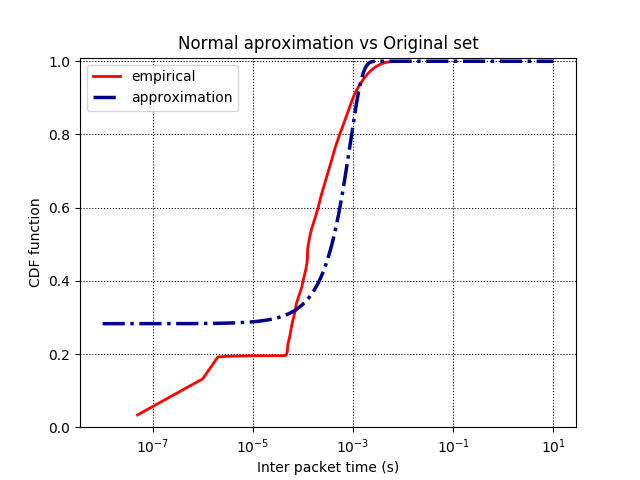
\includegraphics[width=62mm]{figures/apC/cdf/bigFlows_Log_-_Normal_aproximation_vs_Original_set}
	}
	\hspace{0mm}
	\subfloat[Pareto(LR)]{
		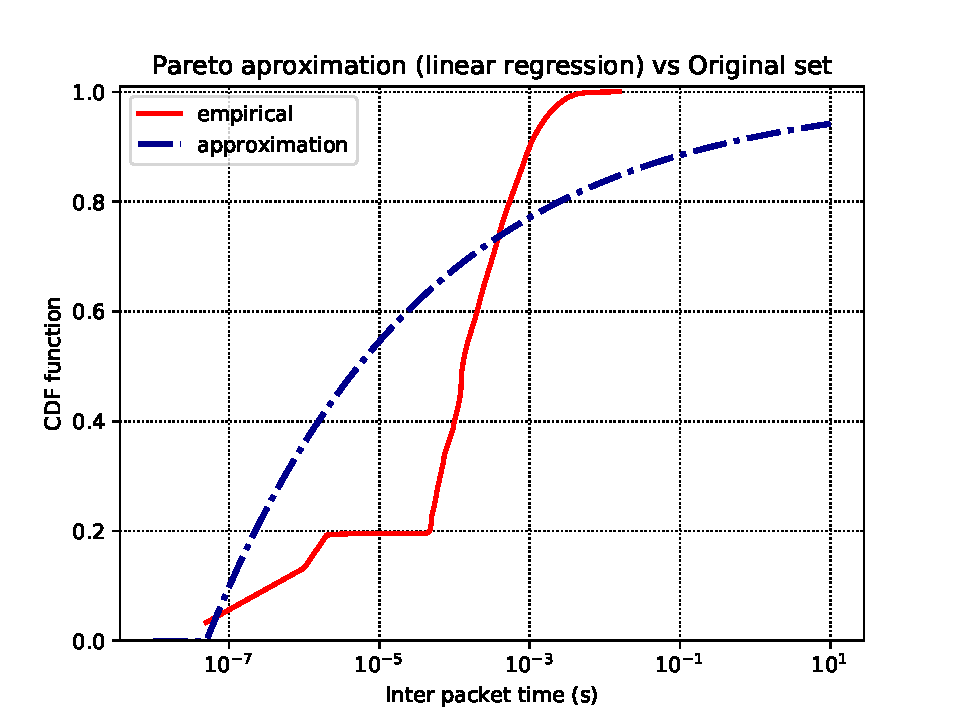
\includegraphics[width=62mm]{figures/apC/cdf/bigFlows_Log_-_Pareto_aproximation_(linear_regression)_vs_Original_set}
	}
	\subfloat[Pareto(MLH)]{
		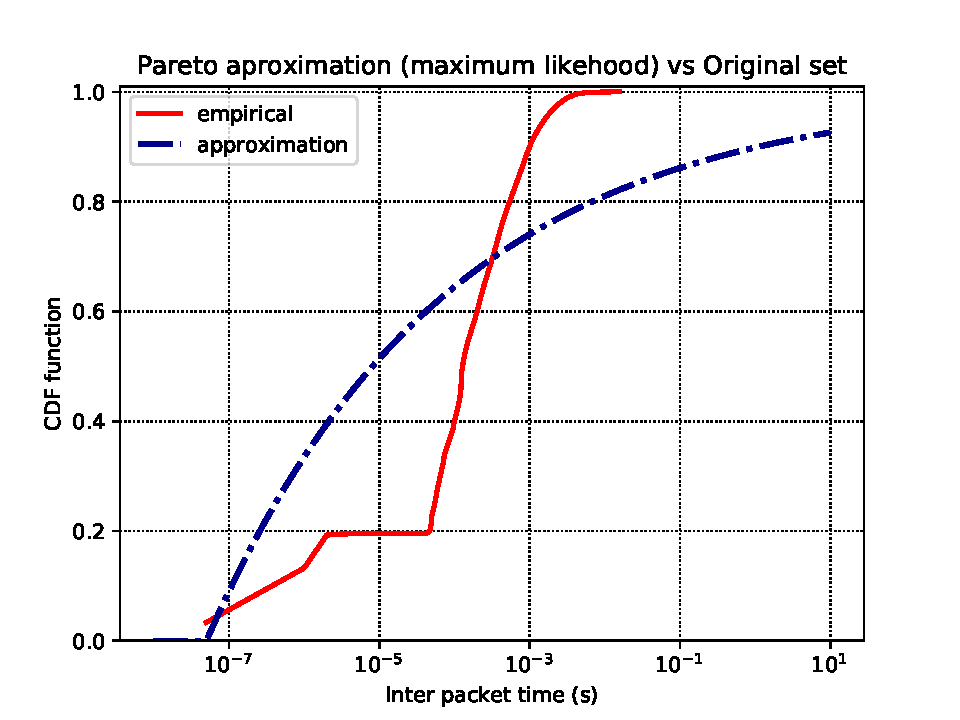
\includegraphics[width=62mm]{figures/apC/cdf/bigFlows_Log_-_Pareto_aproximation_(maximum_likehood)_vs_Original_set}
	}
	\hspace{0mm}
	\subfloat[Weibull]{
		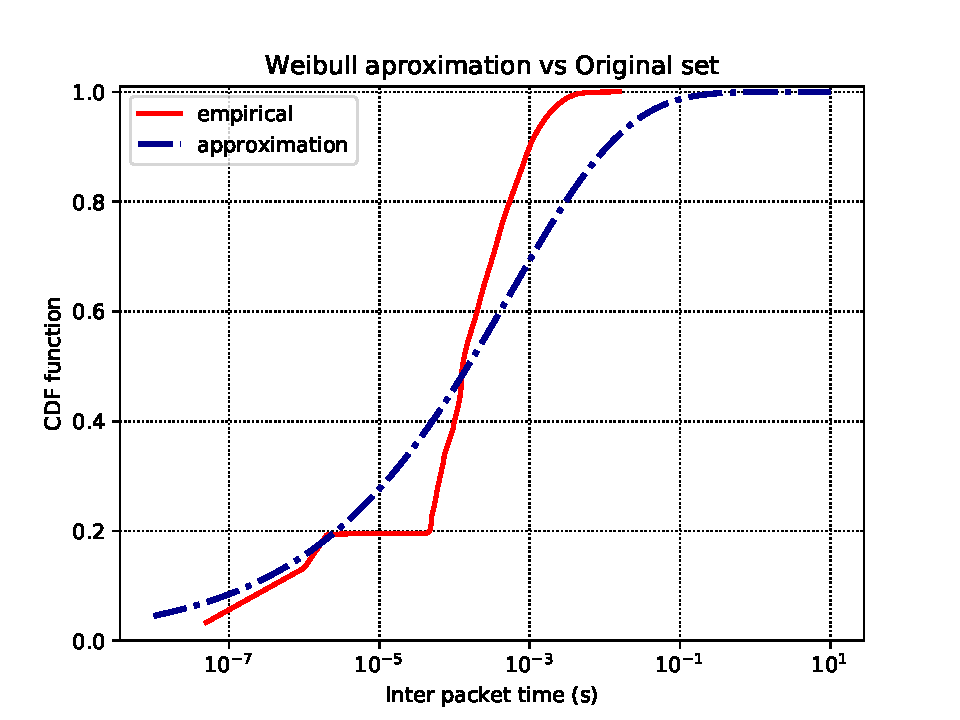
\includegraphics[width=62mm]{figures/apC/cdf/bigFlows_Log_-_Weibull_aproximation_vs_Original_set}
	}
	\caption{CDF functions for the approximations of \textit{lan-gateway-pcap} inter  packet times, of many stochastic functions.}
\end{figure}

\clearpage

\begin{figure}[ht!]
	\centering
	\label{fig:aproximation-original-cdf-wan}
	\subfloat[Chauchy]{
		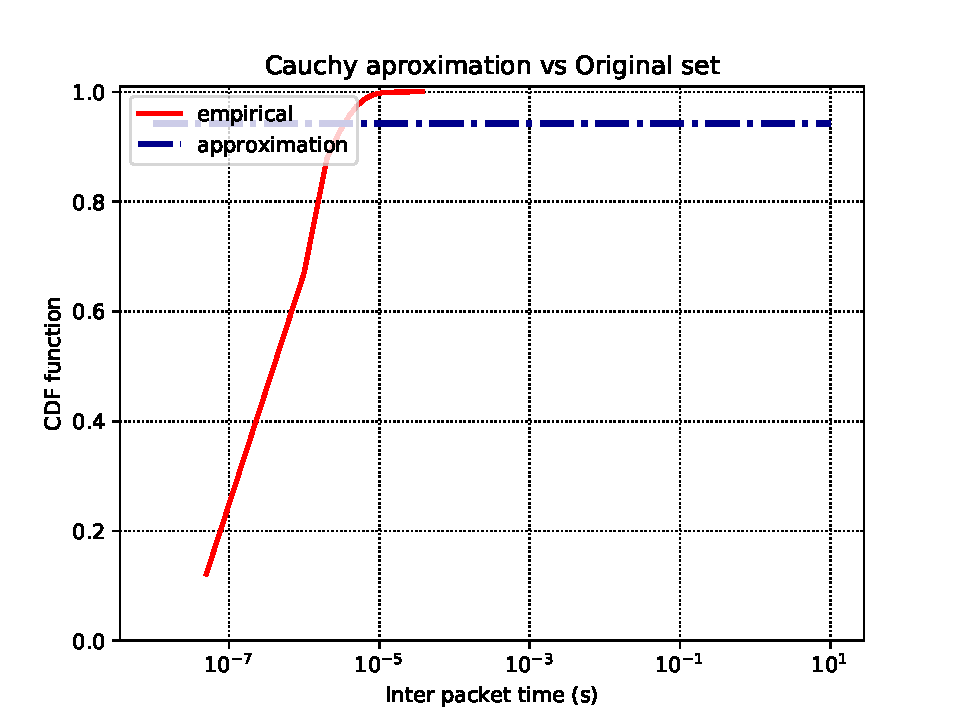
\includegraphics[width=62mm]{figures/apC/cdf/Wan_Log_-_Cauchy_aproximation_vs_Original_set}
	}
	\subfloat[Exponential(LR)]{
		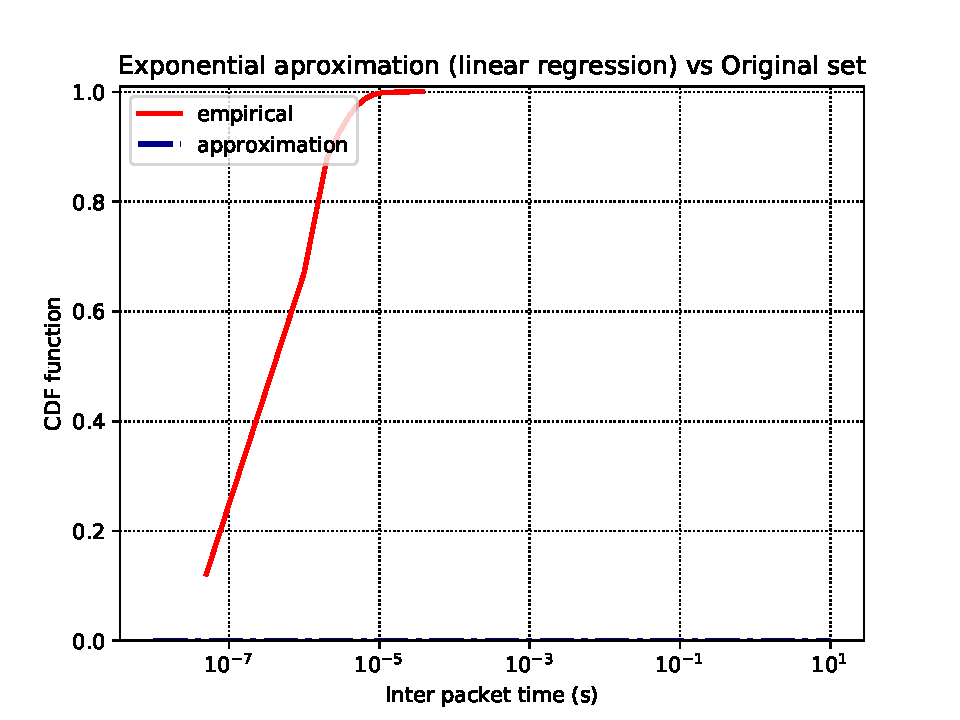
\includegraphics[width=62mm]{figures/apC/cdf/Wan_Log_-_Exponential_aproximation_(linear_regression)_vs_Original_set}
	}
	\hspace{0mm}
	\subfloat[Exponential(Me)]{
		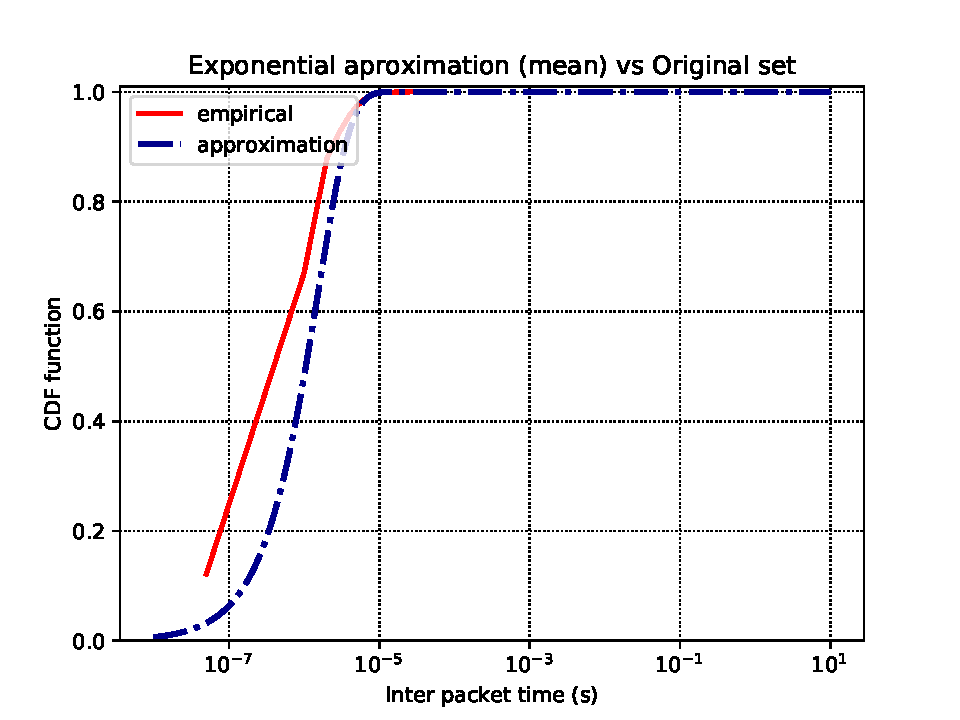
\includegraphics[width=62mm]{figures/apC/cdf/Wan_Log_-_Exponential_aproximation_(mean)_vs_Original_set}
	}
	\subfloat[Normal]{
		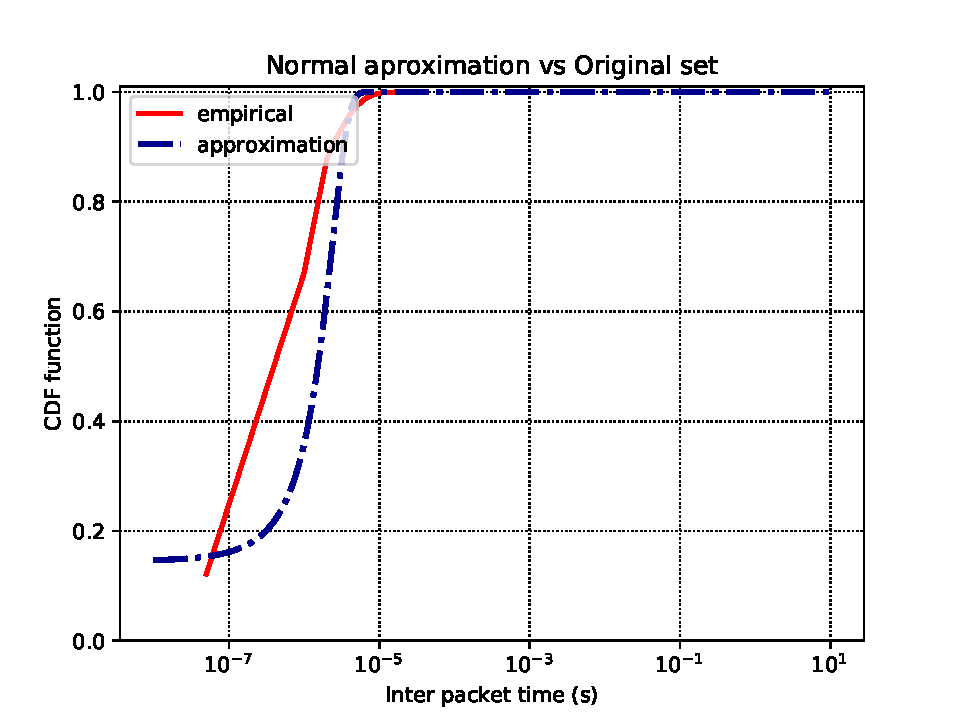
\includegraphics[width=62mm]{figures/apC/cdf/Wan_Log_-_Normal_aproximation_vs_Original_set}
	}
	\hspace{0mm}
	\subfloat[Pareto(LR)]{
		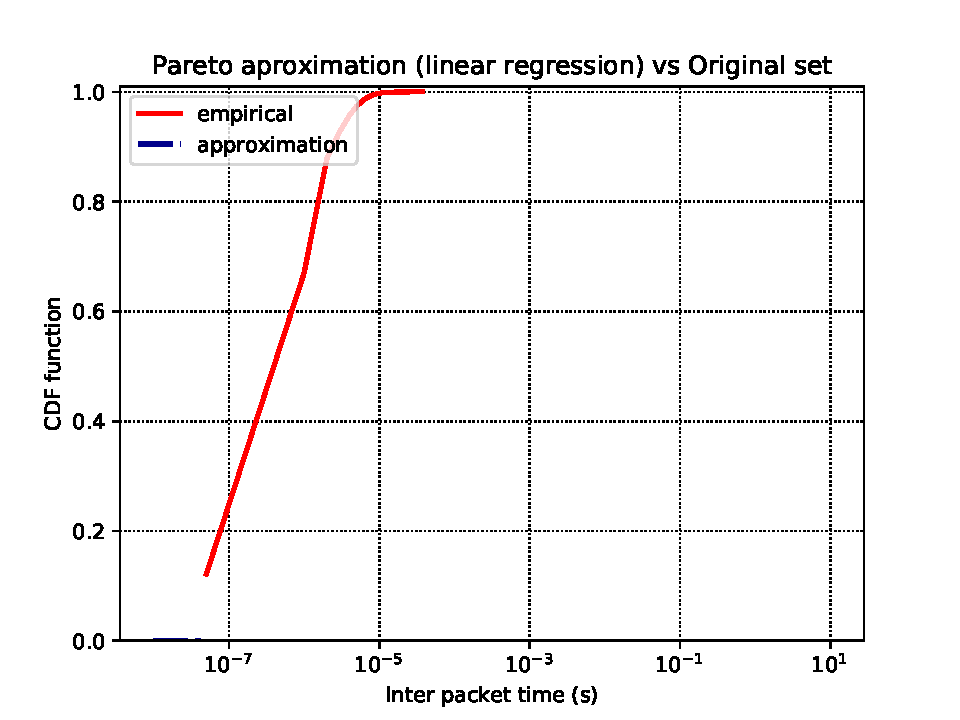
\includegraphics[width=62mm]{figures/apC/cdf/Wan_Log_-_Pareto_aproximation_(linear_regression)_vs_Original_set}
	}
	\subfloat[Pareto(MLH)]{
		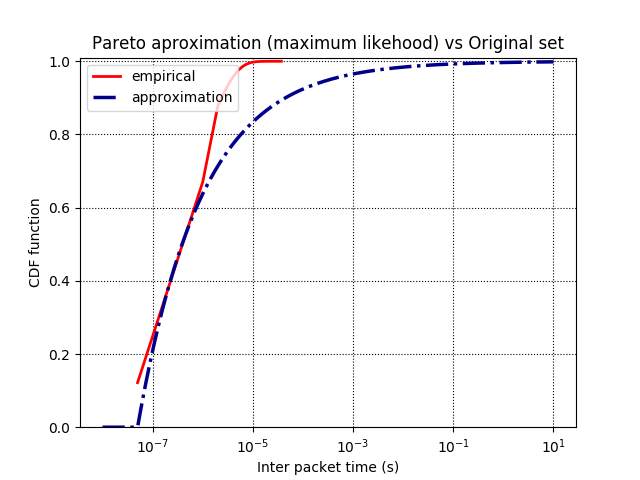
\includegraphics[width=62mm]{figures/apC/cdf/Wan_Log_-_Pareto_aproximation_(maximum_likehood)_vs_Original_set}
	}
	\hspace{0mm}
	\subfloat[Weibull]{
		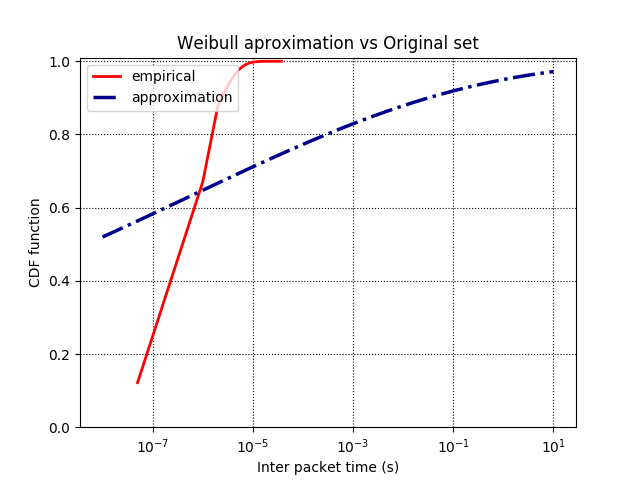
\includegraphics[width=62mm]{figures/apC/cdf/Wan_Log_-_Weibull_aproximation_vs_Original_set}
	}
	\caption{CDF functions for the approximations of \textit{wan-pcap} inter  packet times, of many stochastic functions.}
\end{figure}

\clearpage

\begin{figure}[ht!]
	\centering
	\label{fig:aproximation-original-cdf-lan}
	\subfloat[Chauchy]{
		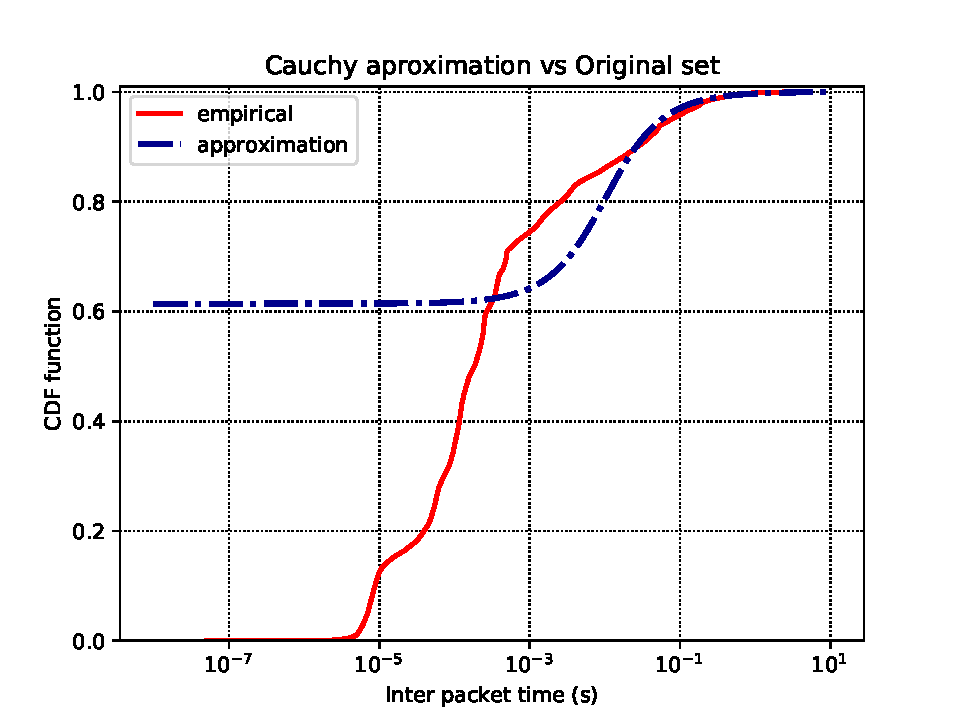
\includegraphics[width=62mm]{figures/apC/cdf/Lan_Log_-_Cauchy_aproximation_vs_Original_set}
	}
	\subfloat[Exponential(LR)]{
		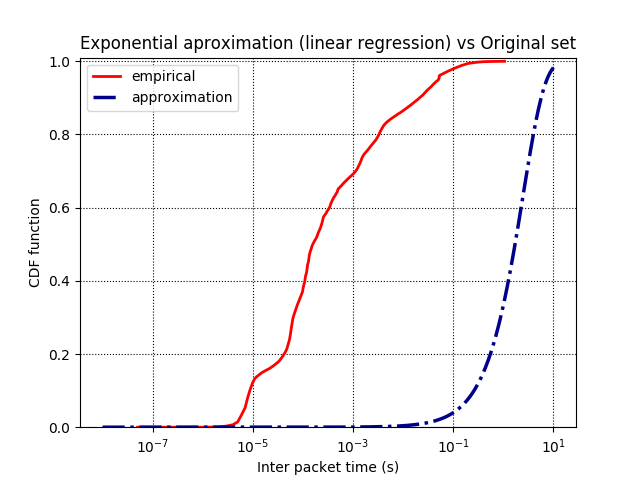
\includegraphics[width=62mm]{figures/apC/cdf/Lan_Log_-_Exponential_aproximation_(linear_regression)_vs_Original_set}
	}
	\hspace{0mm}
	\subfloat[Exponential(Me)]{
		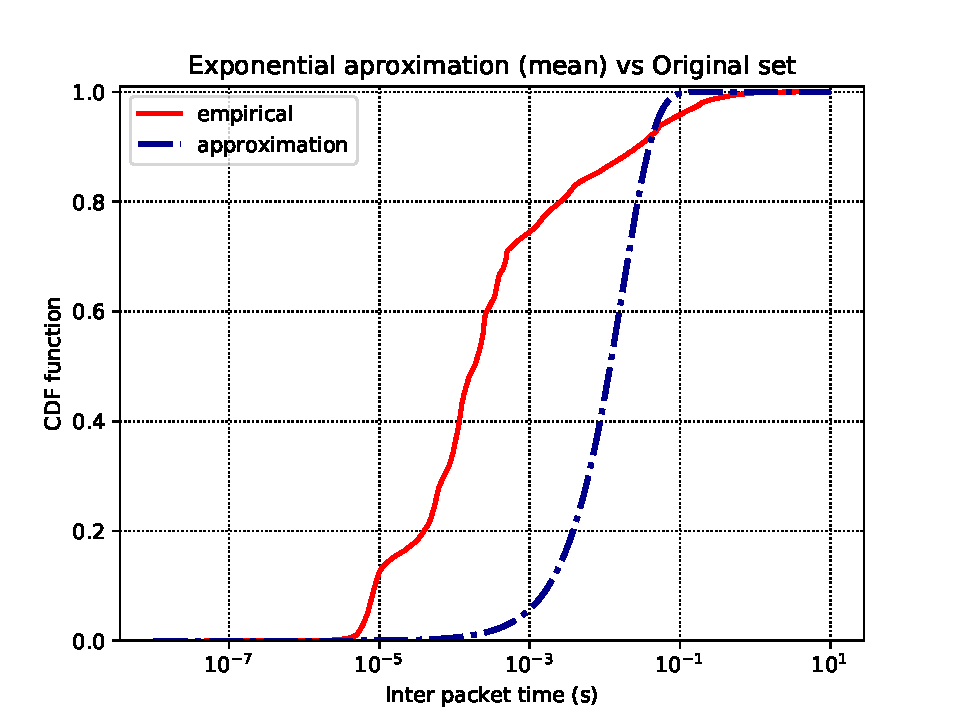
\includegraphics[width=62mm]{figures/apC/cdf/Lan_Log_-_Exponential_aproximation_(mean)_vs_Original_set}
	}
	\subfloat[Normal]{
		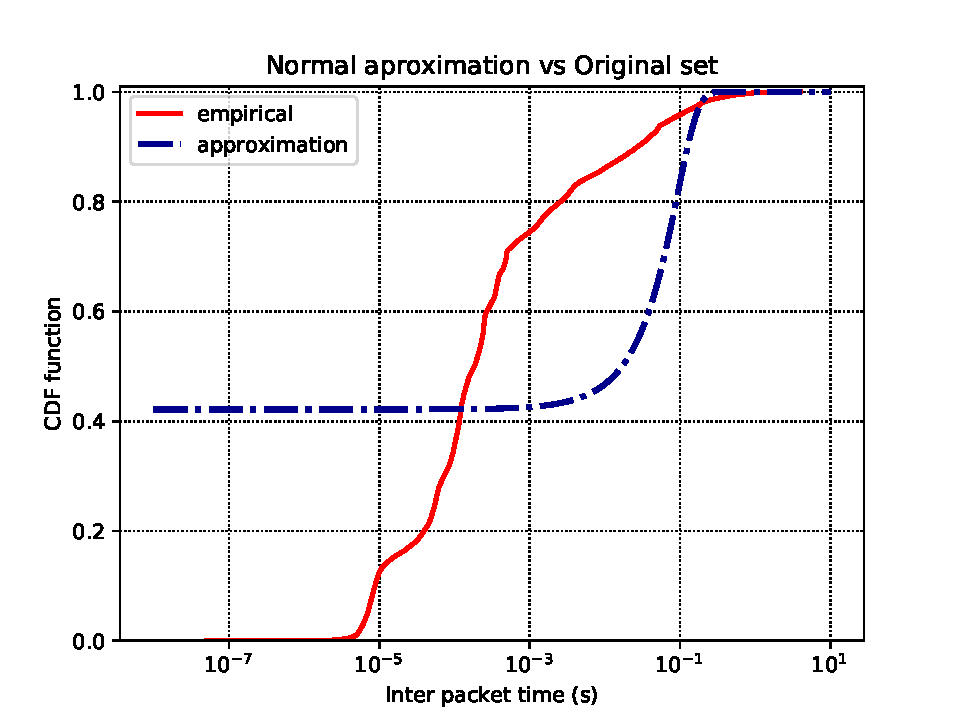
\includegraphics[width=62mm]{figures/apC/cdf/Lan_Log_-_Normal_aproximation_vs_Original_set}
	}
	\hspace{0mm}
	\subfloat[Pareto(LR)]{
		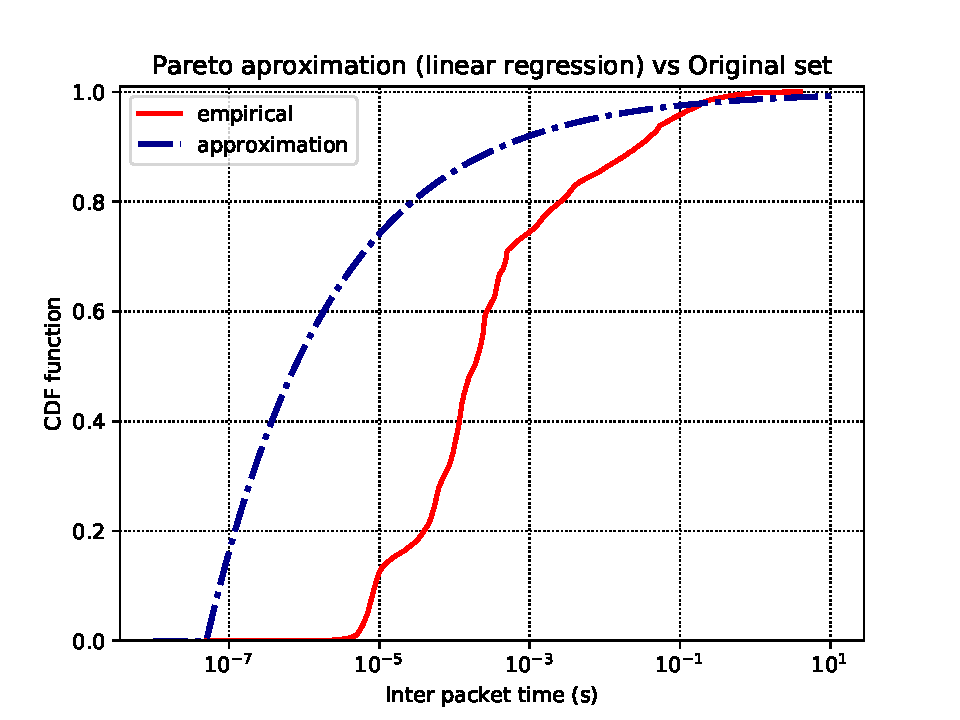
\includegraphics[width=62mm]{figures/apC/cdf/Lan_Log_-_Pareto_aproximation_(linear_regression)_vs_Original_set}
	}
	\subfloat[Pareto(MLH)]{
		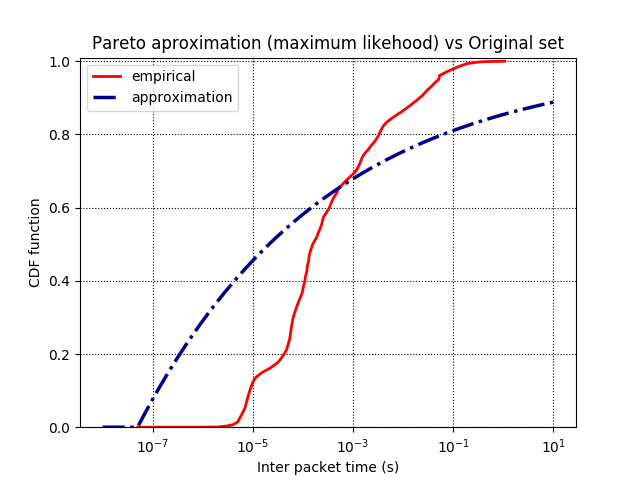
\includegraphics[width=62mm]{figures/apC/cdf/Lan_Log_-_Pareto_aproximation_(maximum_likehood)_vs_Original_set}
	}
	\hspace{0mm}
	\subfloat[Weibull]{
		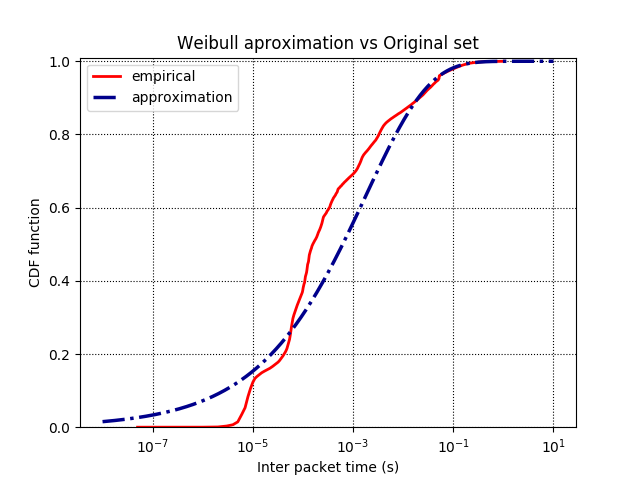
\includegraphics[width=62mm]{figures/apC/cdf/Lan_Log_-_Weibull_aproximation_vs_Original_set}
	}
	\caption{CDF functions for the approximations of \textit{lan-diurnal-firewall-pcap} inter  packet times, of many stochastic functions.}
\end{figure}


%\begin{figure}[ht!]
%	\centering
%	\label{fig:aproximation-original-cdf-skype}
%	\subfloat[Chauchy]{
%		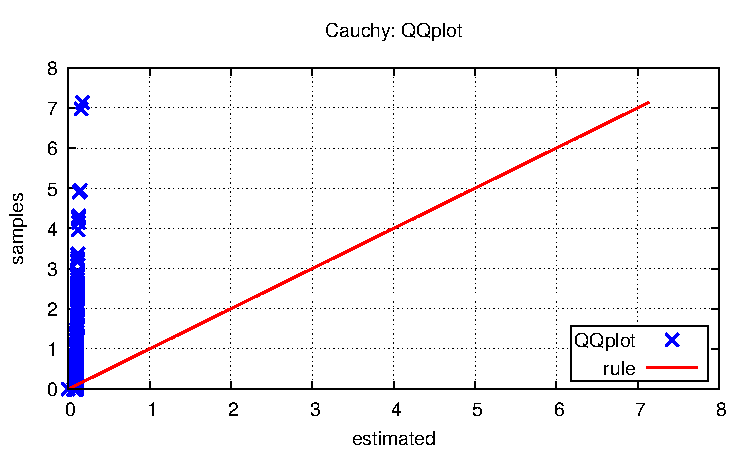
\includegraphics[width=62mm]{figures/apC/qq/skype_QQplot_-_Cauchy}
%	}
%	\subfloat[Exponential(LR)]{
%		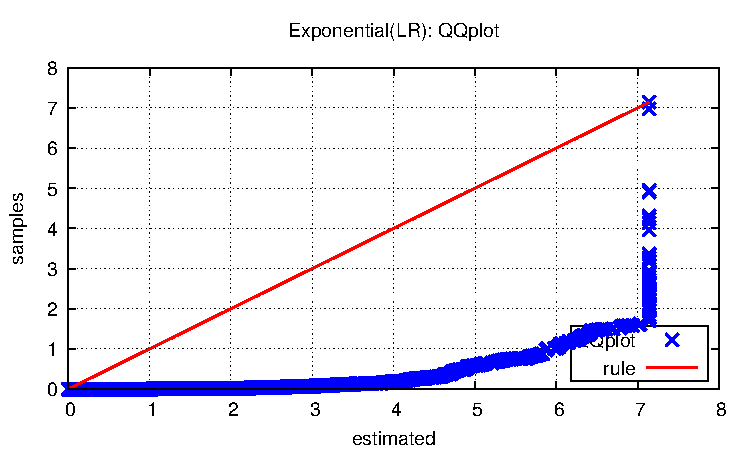
\includegraphics[width=62mm]{figures/apC/qq/skype_QQplot_-_Exponential(LR)}
%	}
%	\hspace{0mm}
%	\subfloat[Exponential(Me)]{
%		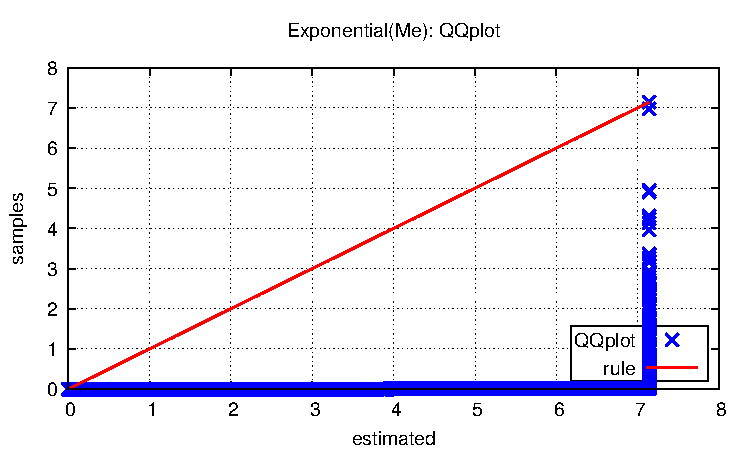
\includegraphics[width=62mm]{figures/apC/qq/skype_QQplot_-_Exponential(Me)}
%	}
%	\subfloat[Normal]{
%		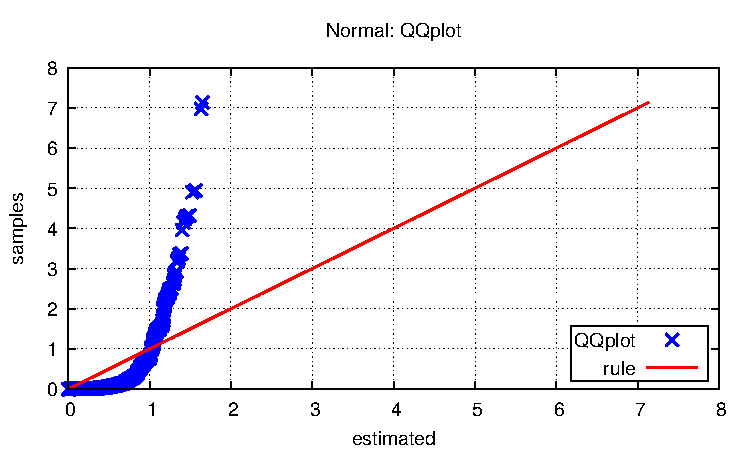
\includegraphics[width=62mm]{figures/apC/qq/skype_QQplot_-_Normal}
%	}
%	\hspace{0mm}
%	\subfloat[Pareto(LR)]{
%		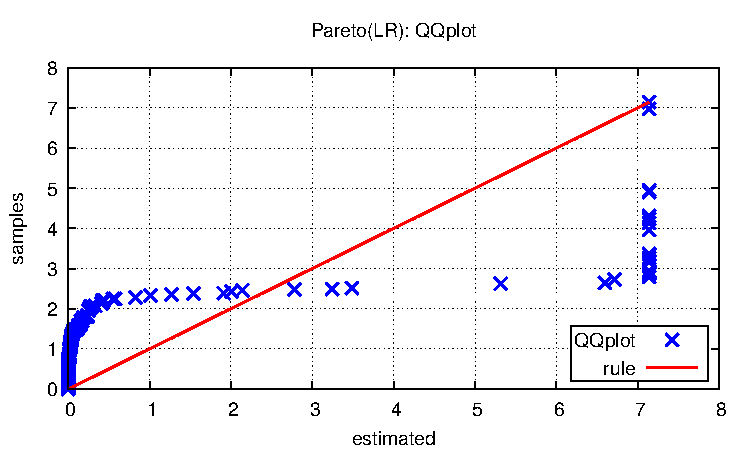
\includegraphics[width=62mm]{figures/apC/qq/skype_QQplot_-_Pareto(LR)}
%	}
%	\subfloat[Pareto(MLH)]{
%		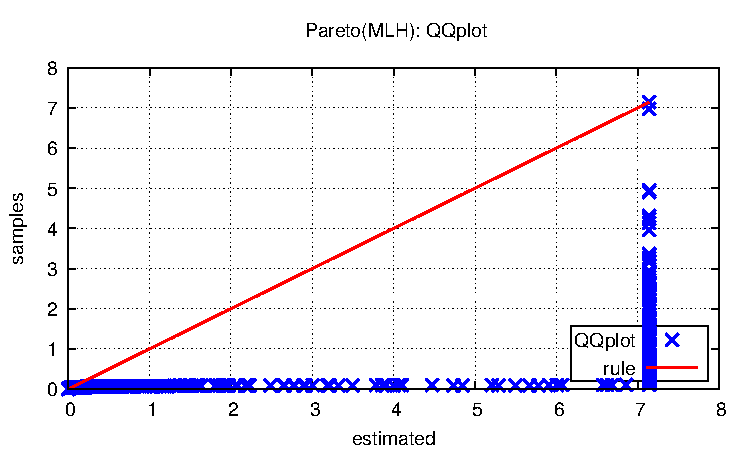
\includegraphics[width=62mm]{figures/apC/qq/skype_QQplot_-_Pareto(MLH)}
%	}
%	\hspace{0mm}
%	\subfloat[Weibull]{
%		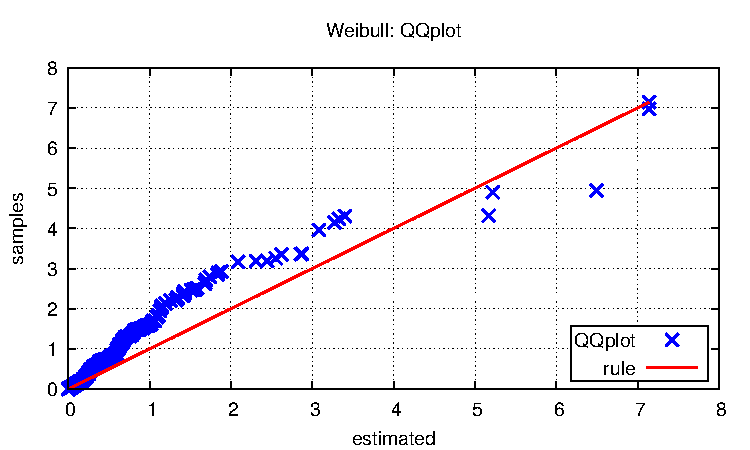
\includegraphics[width=62mm]{figures/apC/qq/skype_QQplot_-_Weibull}
%	}
%	\caption{CDF functions for the approximations of \textit{skype-pcap} inter  packet times, of many stochastic functions.}
%\end{figure}

\clearpage

\begin{figure}[ht!]
	\centering
	\label{fig:qq-bigFlows}
	\subfloat[Chauchy]{
		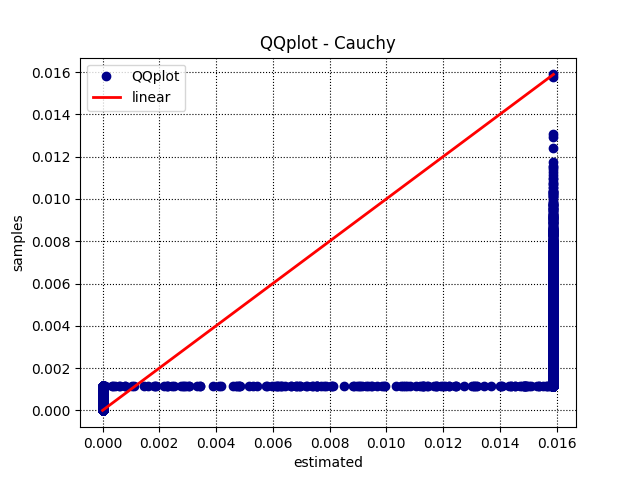
\includegraphics[width=62mm]{figures/apC/qq/bigFlows_QQplot_-_Cauchy}
	}
	\subfloat[Exponential(LR)]{
		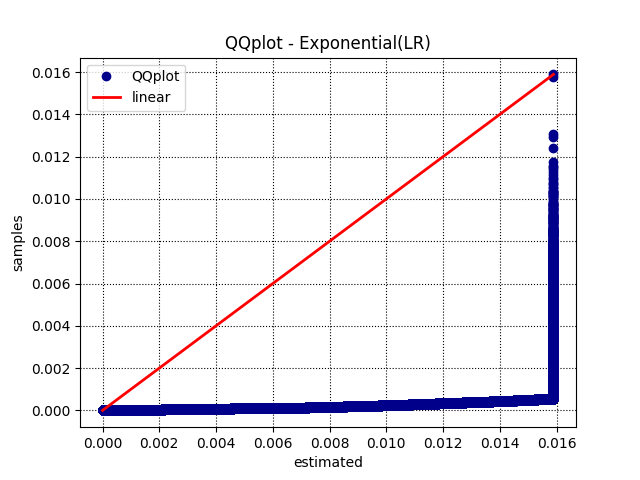
\includegraphics[width=62mm]{figures/apC/qq/bigFlows_QQplot_-_Exponential(LR)}
	}
	\hspace{0mm}
	\subfloat[Exponential(Me)]{
		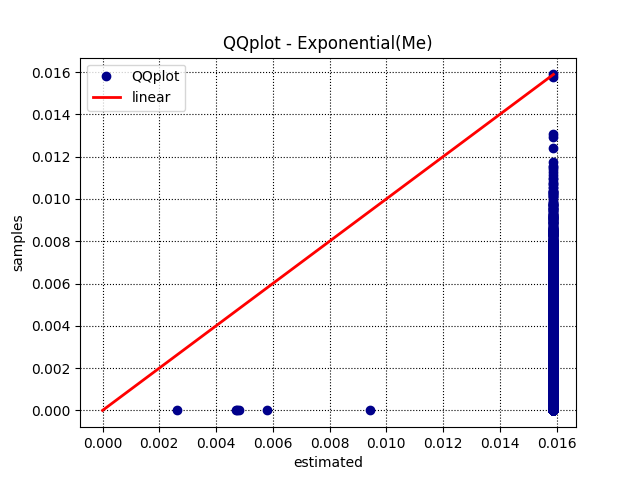
\includegraphics[width=62mm]{figures/apC/qq/bigFlows_QQplot_-_Exponential(Me)}
	}
	\subfloat[Normal]{
		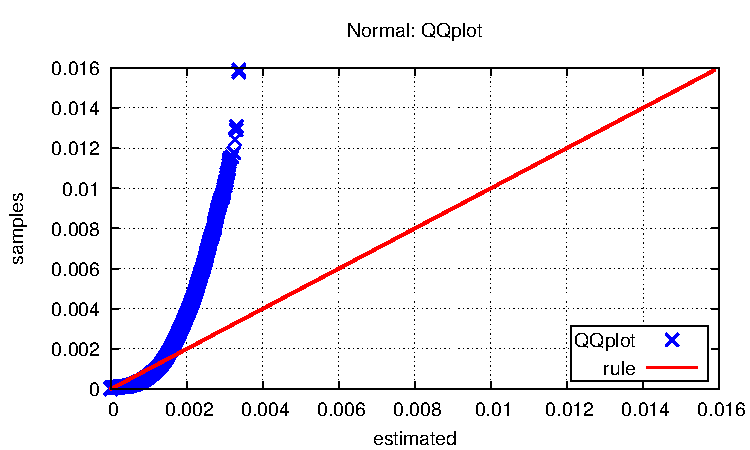
\includegraphics[width=62mm]{figures/apC/qq/bigFlows_QQplot_-_Normal}
	}
	\hspace{0mm}
	\subfloat[Pareto(LR)]{
		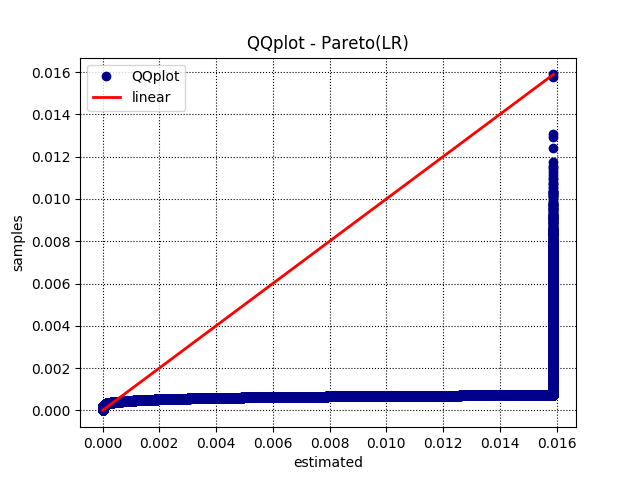
\includegraphics[width=62mm]{figures/apC/qq/bigFlows_QQplot_-_Pareto(LR)}
	}
	\subfloat[Pareto(MLH)]{
		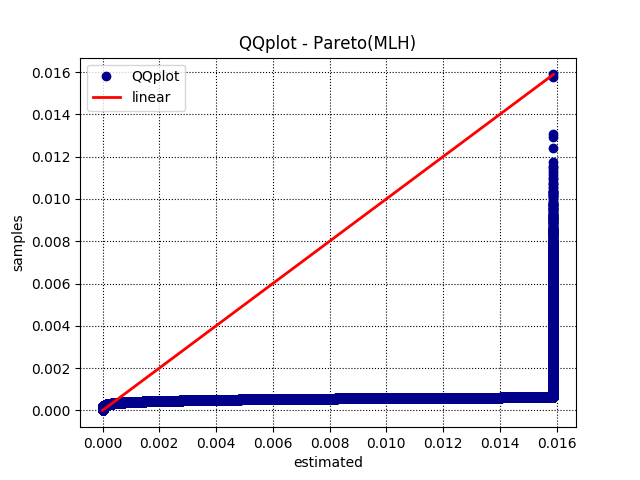
\includegraphics[width=62mm]{figures/apC/qq/bigFlows_QQplot_-_Pareto(MLH)}
	}
	\hspace{0mm}
	\subfloat[Weibull]{
		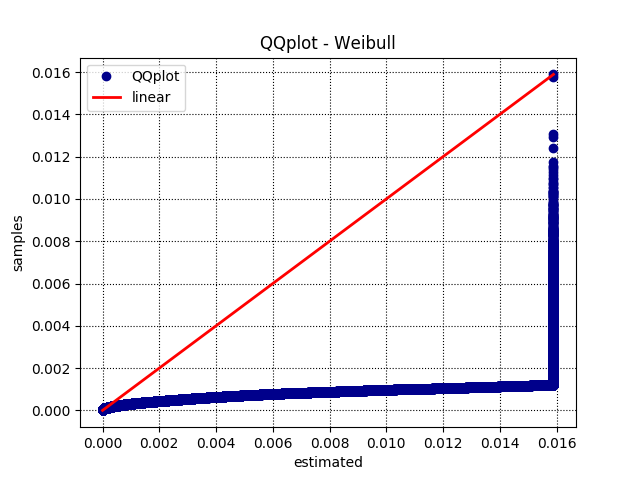
\includegraphics[width=62mm]{figures/apC/qq/bigFlows_QQplot_-_Weibull}
	}
	\caption{CDF functions for the approximations of \textit{lan-gateway-pcap} inter  packet times, of many stochastic functions.}
\end{figure}

\clearpage

\begin{figure}[ht!]
	\centering
	\label{fig:qq-lan}
	\subfloat[Chauchy]{
		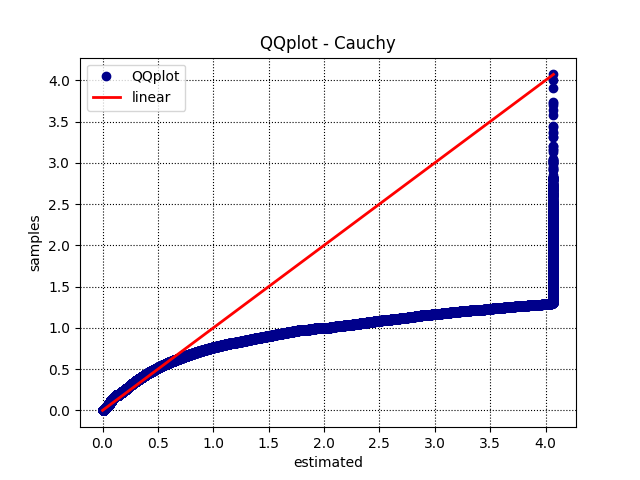
\includegraphics[width=62mm]{figures/apC/qq/Lan_QQplot_-_Cauchy}
	}
	\subfloat[Exponential(LR)]{
		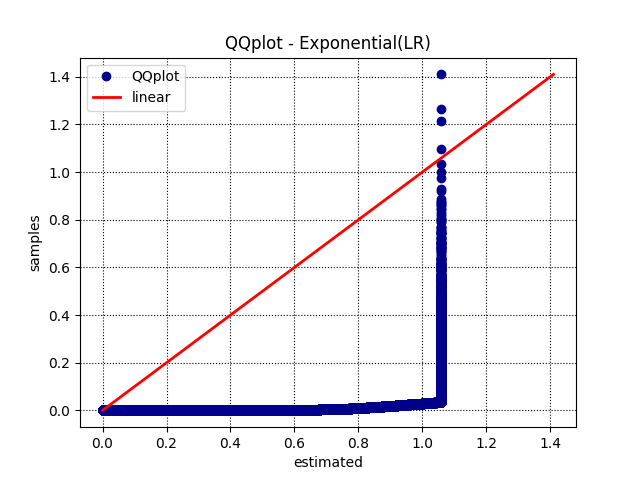
\includegraphics[width=62mm]{figures/apC/qq/Lan_QQplot_-_Exponential(LR)}
	}
	\hspace{0mm}
	\subfloat[Exponential(Me)]{
		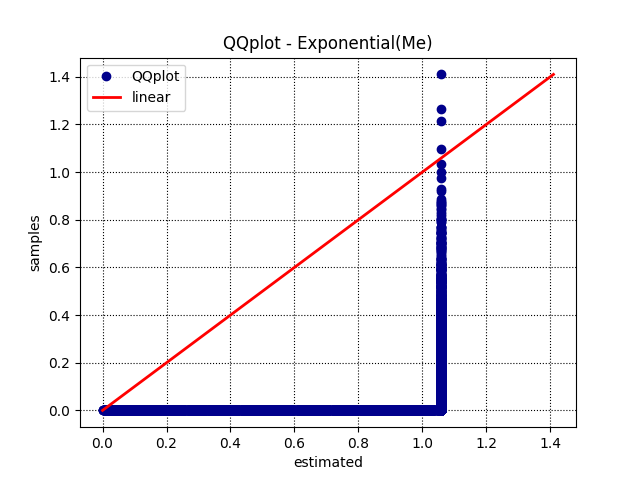
\includegraphics[width=62mm]{figures/apC/qq/Lan_QQplot_-_Exponential(Me)}
	}
	\subfloat[Normal]{
		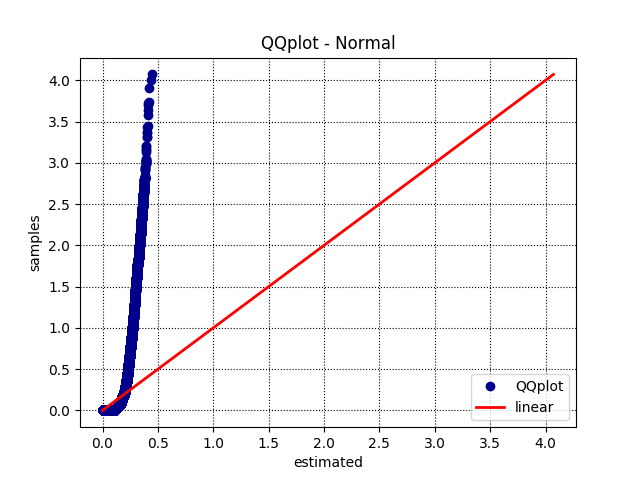
\includegraphics[width=62mm]{figures/apC/qq/Lan_QQplot_-_Normal}
	}
	\hspace{0mm}
	\subfloat[Pareto(LR)]{
		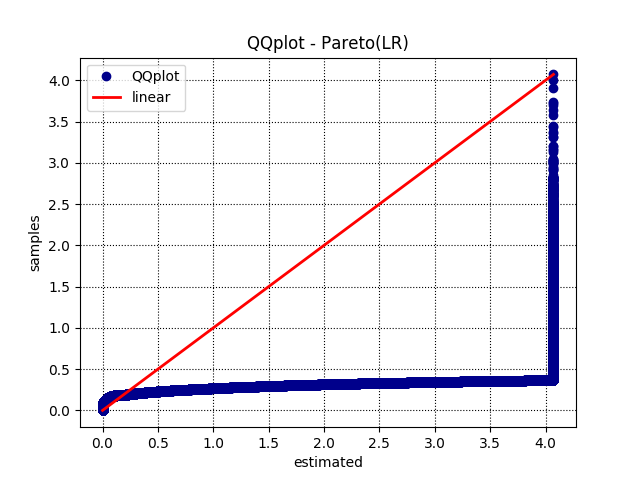
\includegraphics[width=62mm]{figures/apC/qq/Lan_QQplot_-_Pareto(LR)}
	}
	\subfloat[Pareto(MLH)]{
		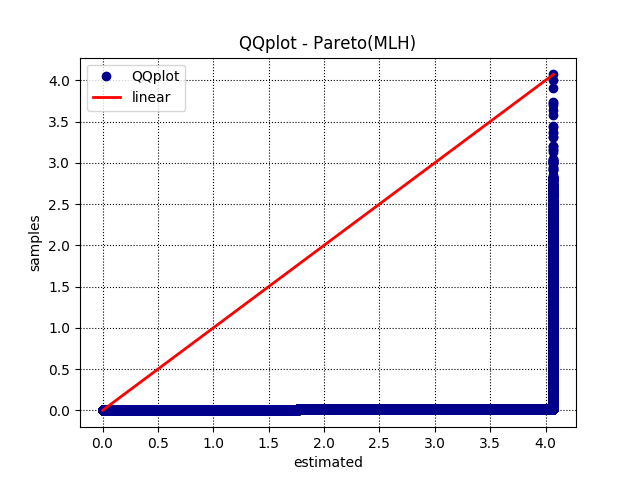
\includegraphics[width=62mm]{figures/apC/qq/Lan_QQplot_-_Pareto(MLH)}
	}
	\hspace{0mm}
	\subfloat[Weibull]{
		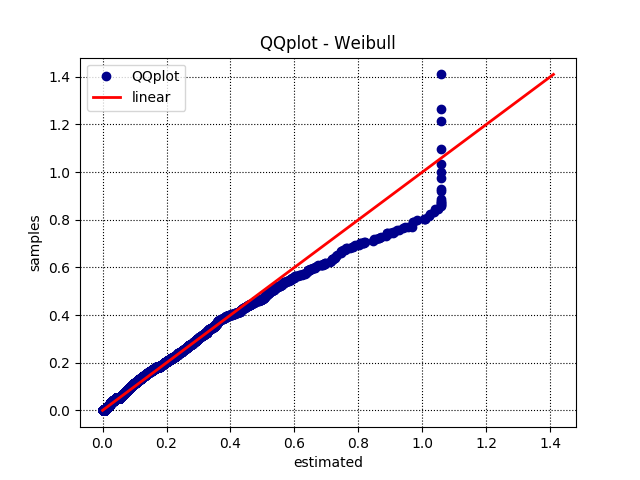
\includegraphics[width=62mm]{figures/apC/qq/Lan_QQplot_-_Weibull}
	}
	\caption{CDF functions for the approximations of \textit{lan-diurnal-firewall-pcap} inter  packet times, of many stochastic functions.}
\end{figure}

\clearpage

\begin{figure}[ht!]
	\centering
	\label{fig:qq-wan}
	\subfloat[Chauchy]{
		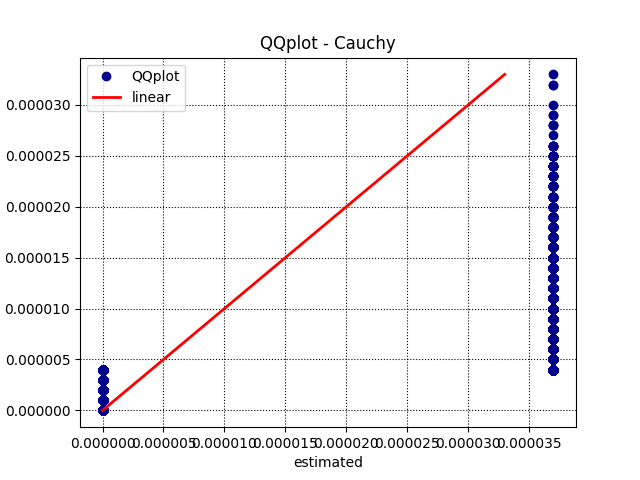
\includegraphics[width=62mm]{figures/apC/qq/Wan_QQplot_-_Cauchy}
	}
	\subfloat[Exponential(LR)]{
		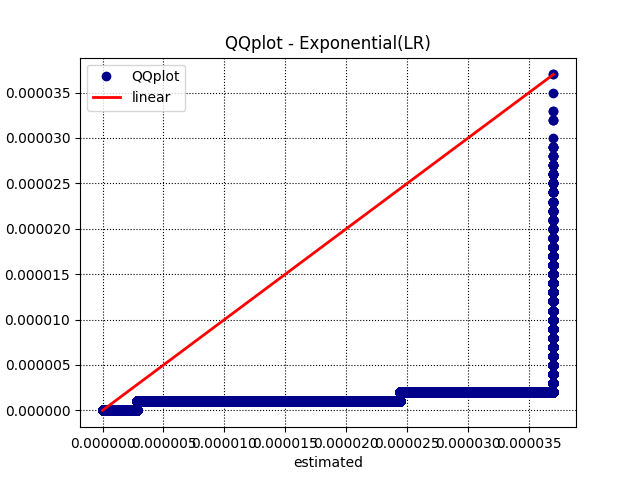
\includegraphics[width=62mm]{figures/apC/qq/Wan_QQplot_-_Exponential(LR)}
	}
	\hspace{0mm}
	\subfloat[Exponential(Me)]{
		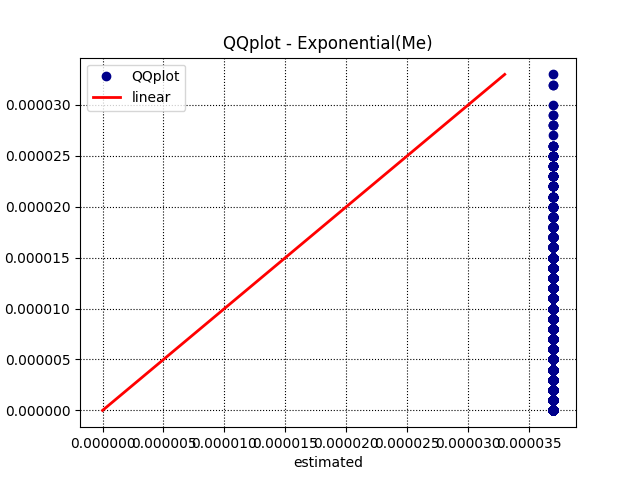
\includegraphics[width=62mm]{figures/apC/qq/Wan_QQplot_-_Exponential(Me)}
	}
	\subfloat[Normal]{
		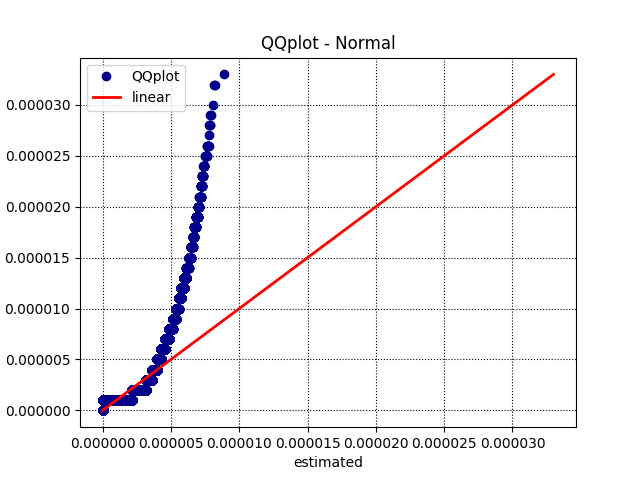
\includegraphics[width=62mm]{figures/apC/qq/Wan_QQplot_-_Normal}
	}
	\hspace{0mm}
	\subfloat[Pareto(LR)]{
		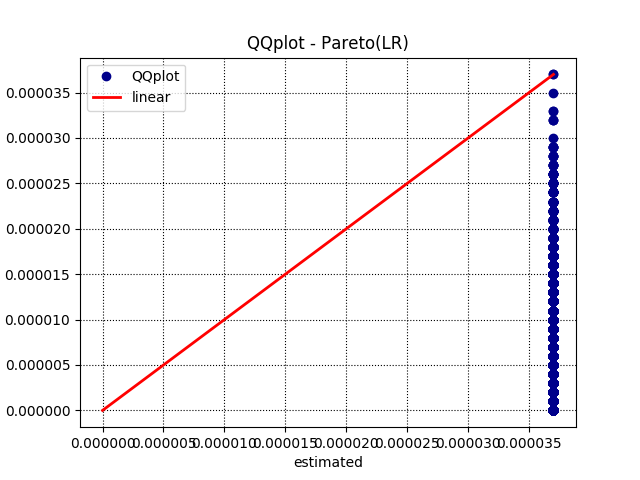
\includegraphics[width=62mm]{figures/apC/qq/Wan_QQplot_-_Pareto(LR)}
	}
	\subfloat[Pareto(MLH)]{
		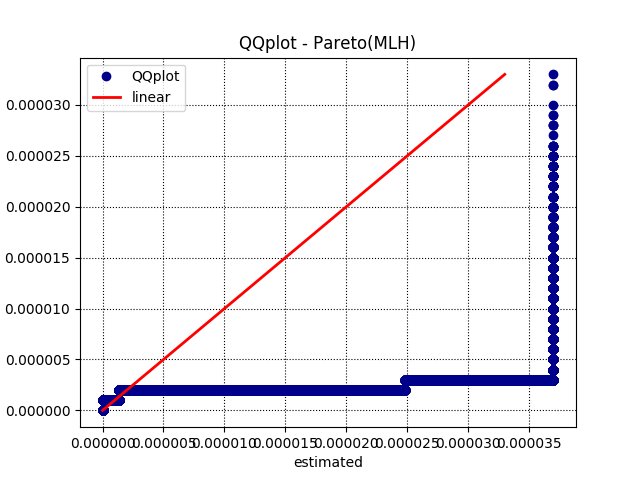
\includegraphics[width=62mm]{figures/apC/qq/Wan_QQplot_-_Pareto(MLH)}
	}
	\hspace{0mm}
	\subfloat[Weibull]{
		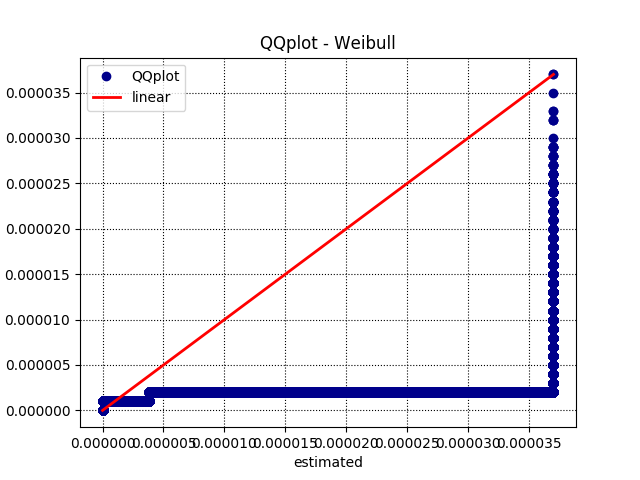
\includegraphics[width=62mm]{figures/apC/qq/Wan_QQplot_-_Weibull}
	}
	\caption{CDF functions for the approximations of \textit{wan-pcap} inter  packet times, of many stochastic functions.}
\end{figure}


\clearpage

%% Skype
\begin{figure}[ht!]
	\centering
	\label{fig:lr-skype}
	\subfloat[Cauchy]{
		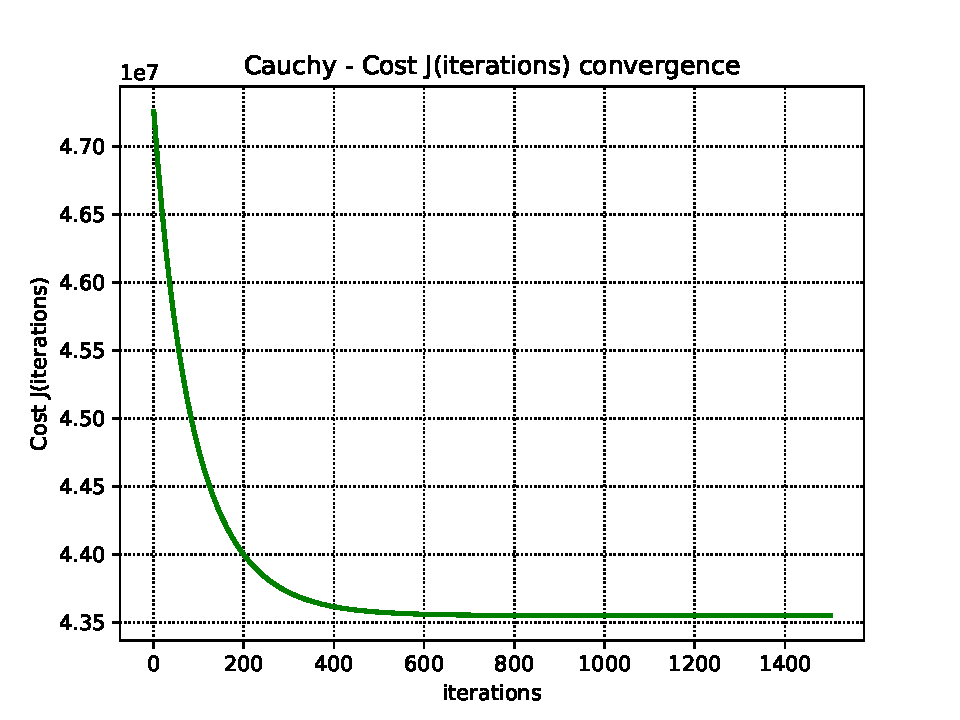
\includegraphics[width=62mm]{figures/apC/lr/Skype_Cauchy_-_Cost_J(iterations)_convergence.pdf}
	}
	\subfloat[Cauchy]{
		\includegraphics[width=62mm]{figures/apC/lr/Skype_Cauchy_-_Linearized_data_and_linear_fitting.png}
	}
	\hspace{0mm}
	\subfloat[Exponential]{
		\includegraphics[width=62mm]{figures/apC/lr/Skype_Exponential_-_Cost_J(iterations)_convergence.pdf}
	}
	\subfloat[Exponential]{
		\includegraphics[width=62mm]{figures/apC/lr/Skype_Exponential_-_Linearized_data_and_linear_fitting.png}
	}
	\hspace{0mm}
	\subfloat[Pareto]{
		\includegraphics[width=62mm]{figures/apC/lr/Skype_Pareto_-_Cost_J(iterations)_convergence.pdf}
	}
	\subfloat[Pareto]{
		\includegraphics[width=62mm]{figures/apC/lr/Skype_Pareto_-_Linearized_data_and_linear_fitting.png}
	}
	\hspace{0mm}
	\subfloat[Weibull]{
		\includegraphics[width=62mm]{figures/apC/lr/Skype_Weibull_-_Cost_J(iterations)_convergence.pdf}
	}
	\subfloat[Weibull]{
		\includegraphics[width=62mm]{figures/apC/lr/Skype_Weibull_-_Linearized_data_and_linear_fitting.png}
	}
	\caption{Data linearization, and linear regression cost history, from gradient descendent for \textit{skype-pcap}.}
\end{figure}


\clearpage

%% bigFlows
\begin{figure}[ht!]
	\centering
	\label{fig:lr-bigFlows}
	\subfloat[Cauchy]{
		\includegraphics[width=62mm]{figures/apC/lr/bigFlows_Cauchy_-_Cost_J(iterations)_convergence.pdf}
	}
	\subfloat[Cauchy]{
		\includegraphics[width=62mm]{figures/apC/lr/bigFlows_Cauchy_-_Linearized_data_and_linear_fitting.png}
	}
	\hspace{0mm}
	\subfloat[Exponential]{
		\includegraphics[width=62mm]{figures/apC/lr/bigFlows_Exponential_-_Cost_J(iterations)_convergence.pdf}
	}
	\subfloat[Exponential]{
		\includegraphics[width=62mm]{figures/apC/lr/bigFlows_Exponential_-_Linearized_data_and_linear_fitting.png}
	}
	\hspace{0mm}
	\subfloat[Pareto]{
		\includegraphics[width=62mm]{figures/apC/lr/bigFlows_Pareto_-_Cost_J(iterations)_convergence.pdf}
	}
	\subfloat[Pareto]{
		\includegraphics[width=62mm]{figures/apC/lr/bigFlows_Pareto_-_Linearized_data_and_linear_fitting.png}
	}
	\hspace{0mm}
	\subfloat[Weibull]{
		\includegraphics[width=62mm]{figures/apC/lr/bigFlows_Weibull_-_Cost_J(iterations)_convergence.pdf}
	}
	\subfloat[Weibull]{
		\includegraphics[width=62mm]{figures/apC/lr/bigFlows_Weibull_-_Linearized_data_and_linear_fitting.png}
	}
	\caption{Data linearization, and linear regression cost history, from gradient descendent for \textit{lan-gateway-pcap}.}
\end{figure}


\clearpage


%% Wan
\begin{figure}[ht!]
	\centering
	\label{fig:lr-wan}
	\subfloat[Cauchy]{
		\includegraphics[width=62mm]{figures/apC/lr/Wan_Cauchy_-_Cost_J(iterations)_convergence.pdf}
	}
	\subfloat[Cauchy]{
		\includegraphics[width=62mm]{figures/apC/lr/Wan_Cauchy_-_Linearized_data_and_linear_fitting.png}
	}
	\hspace{0mm}
	\subfloat[Exponential]{
		\includegraphics[width=62mm]{figures/apC/lr/Wan_Exponential_-_Cost_J(iterations)_convergence.pdf}
	}
	\subfloat[Exponential]{
		\includegraphics[width=62mm]{figures/apC/lr/Wan_Exponential_-_Linearized_data_and_linear_fitting.png}
	}
	\hspace{0mm}
	\subfloat[Pareto]{
		\includegraphics[width=62mm]{figures/apC/lr/Wan_Pareto_-_Cost_J(iterations)_convergence.pdf}
	}
	\subfloat[Pareto]{
		\includegraphics[width=62mm]{figures/apC/lr/Wan_Pareto_-_Linearized_data_and_linear_fitting.png}
	}
	\hspace{0mm}
	\subfloat[Weibull]{
		\includegraphics[width=62mm]{figures/apC/lr/Wan_Weibull_-_Cost_J(iterations)_convergence.pdf}
	}
	\subfloat[Weibull]{
		\includegraphics[width=62mm]{figures/apC/lr/Wan_Weibull_-_Linearized_data_and_linear_fitting.png}
	}
	\caption{Data linearization, and linear regression cost history, from gradient descendent for \textit{wan-pcap}.}
\end{figure}


\clearpage


%% lanDiurnal
\begin{figure}[ht!]
	\centering
	\label{fig:lr-lanDiurnal}
	\subfloat[Cauchy]{
		\includegraphics[width=62mm]{figures/apC/lr/Lan_Cauchy_-_Cost_J(iterations)_convergence.pdf}
	}
	\subfloat[Cauchy]{
		\includegraphics[width=62mm]{figures/apC/lr/Lan_Cauchy_-_Linearized_data_and_linear_fitting.png}
	}
	\hspace{0mm}
	\subfloat[Exponential]{
		\includegraphics[width=62mm]{figures/apC/lr/Lan_Exponential_-_Cost_J(iterations)_convergence.pdf}
	}
	\subfloat[Exponential]{
		\includegraphics[width=62mm]{figures/apC/lr/Lan_Exponential_-_Linearized_data_and_linear_fitting.png}
	}
	\hspace{0mm}
	\subfloat[Pareto]{
		\includegraphics[width=62mm]{figures/apC/lr/Lan_Pareto_-_Cost_J(iterations)_convergence.pdf}
	}
	\subfloat[Pareto]{
		\includegraphics[width=62mm]{figures/apC/lr/Lan_Pareto_-_Linearized_data_and_linear_fitting.png}
	}
	\hspace{0mm}
	\subfloat[Weibull]{
		\includegraphics[width=62mm]{figures/apC/lr/Lan_Weibull_-_Cost_J(iterations)_convergence.pdf}
	}
	\subfloat[Weibull]{
		\includegraphics[width=62mm]{figures/apC/lr/Lan_Weibull_-_Linearized_data_and_linear_fitting.png}
	}
	\caption{Data linearization, and linear regression cost history, from gradient descendent for \textit{lan-firewall-pcap}.}
\end{figure}


\clearpage


\begin{figure}[ht!]
%%%%%%%%%%%%%%%%%%%%%%%
% AIC / BIC logscale
%%%%%%%%%%%%%%%%%%%%%%%
\begin{figure}[H]
\centering
\includegraphics[scale=0.5]{figures/apC/rm/aic-bic-logscale-sumary.eps}
\caption{$AIC$ and $BIC$ summary for all the traces, presented in log scale.}
\label{fig:aic-bic-summary-logscale}
\end{figure}
%%%%%%%%%%%%%%%%%%%%%%%
% AIC / BIC order
%%%%%%%%%%%%%%%%%%%%%%%
\begin{figure}[H]
\centering
\includegraphics[scale=0.5]{figures/apC/rm/aic-bic-order.eps}
\caption{$AIC$ and $BIC$ summary for all the traces, presenting the order.}
\label{fig:aic-bic-order-old}
\end{figure}
%%%%%%%%%%%%%%%%%%%%%%%
% Cost function summary
%%%%%%%%%%%%%%%%%%%%%%%
\begin{figure}[H]
\centering
\includegraphics[scale=0.5]{figures/apC/rm/cost-function-summary.eps}
\caption{Cost function $J_M$ summary.}
\label{fig:cost-function-summary}
\end{figure}
\end{figure}

\clearpage
